\chapter{Experimental Evaluation}
\label{ch:experimental_evaluation}

This chapter evaluates the resulting systems under a fixed experimental protocol,
the goal is to compare the behaviour of the Flink Strategy Engine, Batch XGBoost, and the MOA Online Learner on the same pit decision contracts.

The evaluation is organized around the two targets introduced earlier: \texttt{pit\_any\_h2}, which measures whether a pit stop is predicted within the evaluation
horizon, and \texttt{pit\_success\_h2}, which measures whether a successful evaluated pit stop is predicted. The chapter first defines the frozen protocol, then reports
the rule engine baseline, the training and runtime characteristics of the learning branches, the headline comparison for pit timing, and the stricter comparison for successful
pit calls.
% The final part discusses diagnostic views that help interpret the differences between operational precision, event coverage, and matched-pit success rate.

\section{Evaluation Scope and Frozen Protocol}

Before presenting the results, the evaluation protocol is fixed explicitly. This is necessary because the systems do not produce the same type of output and do not naturally
operate on identical tables as described in Chapter \ref{ch:problem_solving} Section \ref{sec:corrections}. The Flink Strategy Engine emits rule based recommendation labels,
Batch XGBoost emits out-of-fold probability scores, and MOA emits vote based scores
in prequential order. The protocol defines how these outputs are converted into comparable positive calls and how those calls are matched against truth.
All headline results are computed on seasons 2022--2025, which is the ground effect F1 car era. The truth universe mode is \texttt{canonical\_sde\_truth}, and the main lens is \texttt{clean\_actionable}. This means
that the comparison uses the shared SDE-defined truth universe and removes cases that are not considered fair actionable strategy decisions under the clean lens. By doing so
comparing systems on different race, driver, or event populations is avoided.

Two targets are evaluated. The first target, \texttt{pit\_any\_h2}, measures pit timing: a positive call is correct when an eligible pit stop is matched within the timing
contract. The second target, \texttt{pit\_success\_h2}, measures successful pit-call prediction: a positive call is correct only when an eligible future pit stop is matched
and the post pit evaluator classifies that stop as successful. For this second contract, failed or disadvantage pit outcomes are treated as negatives, while unresolved,
weather related, and unmapped outcomes are excluded from the clean success truth.
Both are described at \ref{ch:problem_framing} Section \ref{sec:contracts}.

The compared systems are:
\begin{itemize}
    \item the frozen Flink Strategy Engine profile
    \item Batch XGBoost with the No-Year feature profile
    \item Batch XGBoost with the Percent feature profile
    \item MOA Online Learner with the No-Year feature profile
    \item MOA Online Learner with the Percent feature profile
\end{itemize}

The Batch systems are evaluated with race sequential out-of-fold predictions. Each score is produced on a race that was not used in the corresponding training prefix.
The MOA systems are evaluated with the prequential test-then-train protocol where each row is predicted first and then used for learning. The Flink Strategy Engine is evaluated
from its persisted \texttt{pit\_suggestions} artifacts, with the selected frozen rule profile.

The evaluation artifacts were also checked for protocol consistency before reporting the results. In particular, the \texttt{pit\_success\_h2} evaluation uses the corrected success
contract: a positive call is matched only against future pit evidence, positive calls from the system without a real match are counted as false positives,
and matched-pit success rate is kept only as a diagnostic measure.
This distinction is important because successful pit call prediction is stricter than pit timing,
counting these no match calls as false positives gives a more realistic operational view of the system behaviour.



\section{Flink Strategy Engine Baseline and Freeze Decision}

As described in Section~\ref{sec:flink_tuning}, the Flink Strategy Engine was not used in its first rule configuration. Several deterministic variants were tested before
comparing the rule based system with Batch XGBoost and MOA. This step was needed to obtain a stable rule baseline, while keeping the later comparison independent from the
tuning of the learning models.

The first variant was the strict profile. In this configuration, the engine mainly relied on the base score, timing gates, and actionability gates. Optional promotion
mechanisms were disabled, especially the rival pressure promotion. This made the system conservative: it emitted fewer strong pit calls and avoided some noisy recommendations,
but it also missed situations where nearby rivals created a relevant strategic pressure.

The second variant enabled rival pressure. In this configuration, recent pit activity from nearby rivals could promote a near actionable situation into a stronger
recommendation. The objective was to increase the reach of the Flink Strategy Engine, especially in cases where waiting could lose a strategic window. This improved recall, but
it also introduced more noisy calls.

The final variant kept the rival pressure mechanism but added guards. Promotions were allowed only when the surrounding context supported the call, for example through
timing pressure, urgency, recent lap constraints, and gap conditions. This guarded profile was selected as the frozen Flink Strategy Engine baseline. After this point, the
rule engine configuration was kept fixed and the Batch and MOA systems were compared against it under the same evaluation protocol.

Table~\ref{tab:flink_strategy_engine_freeze} summarizes the tuning trajectory. The strict profile is the most conservative one. The rival pressure profile increases reach,
but loses precision. The frozen guarded profile recovers precision while keeping the same $F_{0.5}$ value as the rival pressure configuration.

\begin{table}[htbp]
    \centering
    \caption{Flink Strategy Engine variant comparison before freezing the deterministic baseline.}
    \label{tab:flink_strategy_engine_freeze}
    \begin{tabular}{lcccl}
        \toprule
        Variant               & Precision & Recall & $F_{0.5}$ & Interpretation                       \\
        \midrule
        Strict                & 0.232     & 0.068  & 0.156     & Stable but conservative              \\
        Rival pressure        & 0.218     & 0.097  & 0.174     & Better reach, more noise             \\
        Flink Strategy Engine & 0.248     & 0.079  & 0.174     & Recovered precision, equal $F_{0.5}$ \\
        \bottomrule
    \end{tabular}
\end{table}

The selected profile is the deterministic baseline obtained from the rule engine tuning stage.
The following sections use this frozen Flink Strategy Engine when comparing the three decision paradigms.

\begin{figure}[htbp]
    \centering
    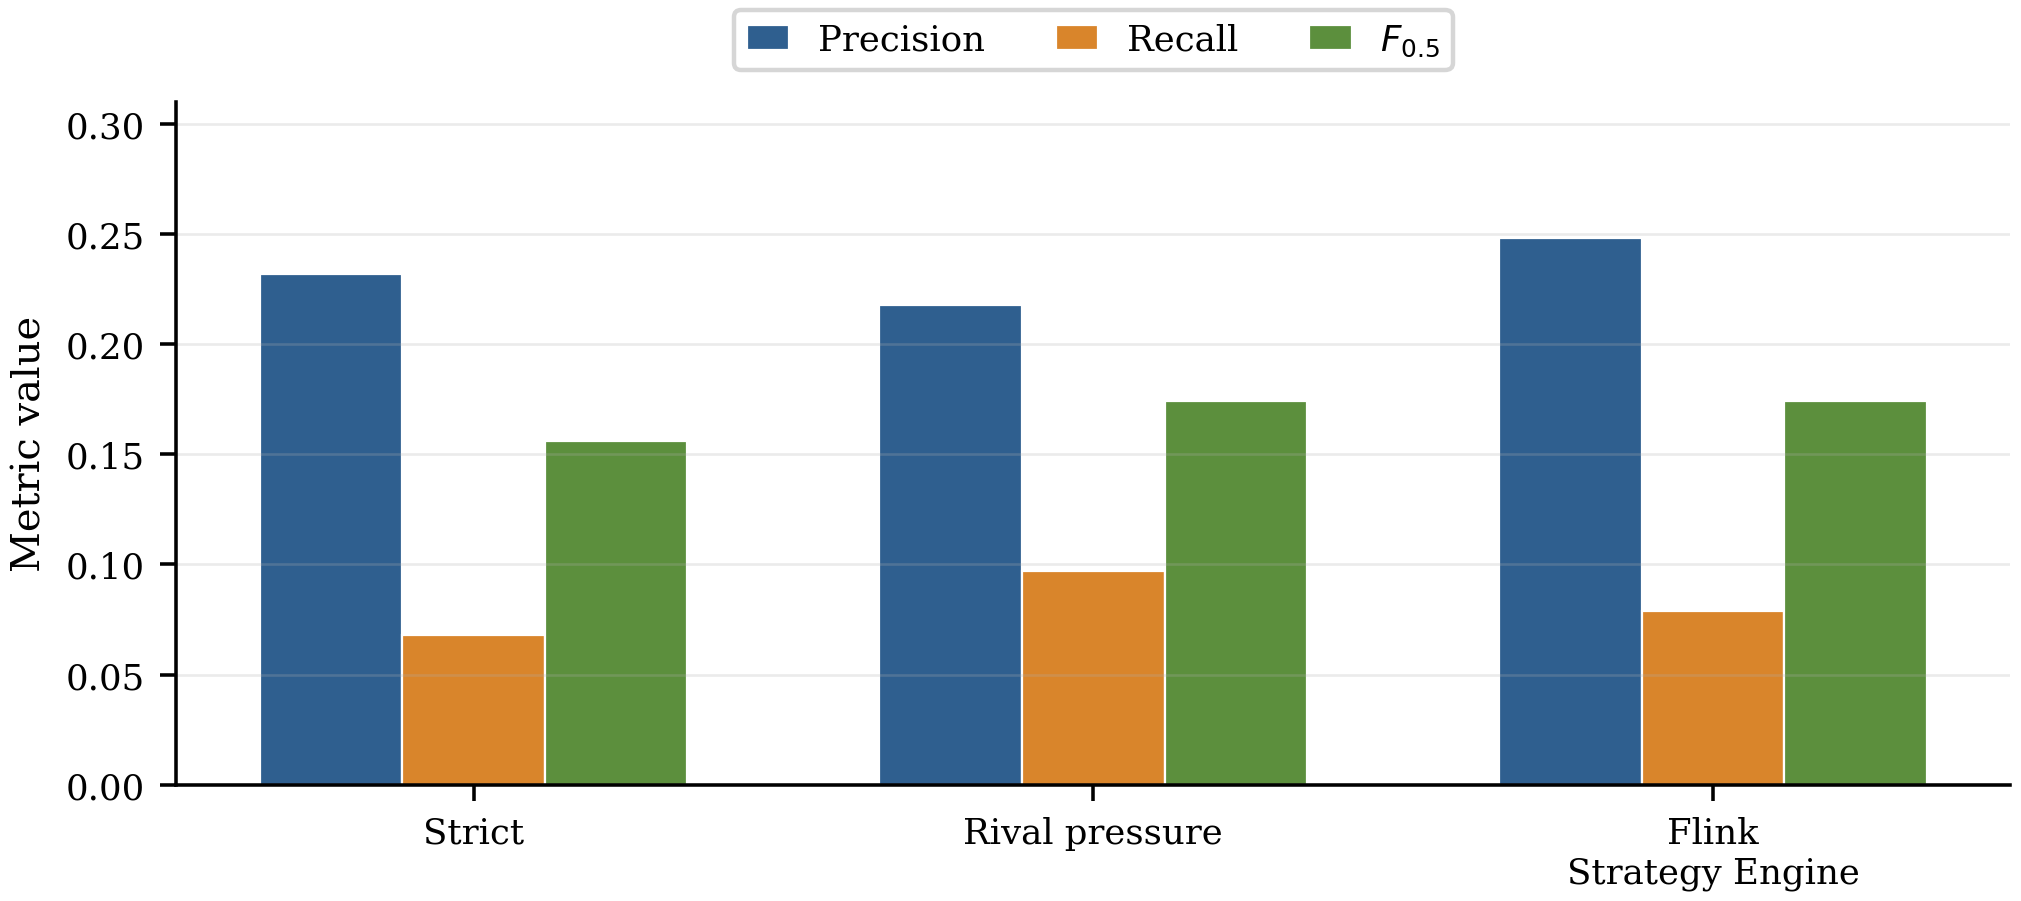
\includegraphics[width=0.98\textwidth]{Images/ch5/rule_engine_tuning_variants_clean.png}
    \caption{Rule-engine tuning summary for 2025 under the clean\_actionable lens, showing pit\_any\_h2 precision, recall, and $F_{0.5}$ across the three rule-engine variants.}
    \label{fig:rule_engine_tuning_variants_clean}
\end{figure}

\section{Training Runtime Comparison}

The first experimental comparison concerns the runtime of the two learning branches. The values in Table~\ref{tab:training_runtime_comparison} report the learner runtime for
each profile and target. Dataset preparation and MOA export are treated as separate stages and are not included in these times.

The difference between Batch and MOA is expected from the evaluation protocols described in Chapter~\ref{ch:problem_solving}. Batch XGBoost uses race-sequential out-of-fold
evaluation: the model is trained on the previous races, tested on the next held-out race, then trained again on a larger prefix and tested on the following race. This repeated
fitting makes the Batch branch slower. MOA instead runs once over the exported stream in prequential order. Each instance is predicted and then used for training, so
the learner processes the stream in a single pass.

\begin{table}[htbp]
    \centering
    \caption{Training and evaluation runtime by learner, feature profile, and target.}
    \label{tab:training_runtime_comparison}
    \begin{tabular}{lll}
        \toprule
        System        & Target                    & Runtime \\
        \midrule
        Batch No-Year & \texttt{pit\_any\_h2}     & 1m 44s  \\
        Batch No-Year & \texttt{pit\_success\_h2} & 1m 41s  \\
        Batch Percent & \texttt{pit\_any\_h2}     & 1m 38s  \\
        Batch Percent & \texttt{pit\_success\_h2} & 1m 29s  \\
        MOA No-Year   & \texttt{pit\_any\_h2}     & 24s     \\
        MOA No-Year   & \texttt{pit\_success\_h2} & 20s     \\
        MOA Percent   & \texttt{pit\_any\_h2}     & 18s     \\
        MOA Percent   & \texttt{pit\_success\_h2} & 13s     \\
        \bottomrule
    \end{tabular}
\end{table}

The timing results should therefore be interpreted as runtime evidence for the selected evaluation implementation, not as a general benchmark of
XGBoost against MOA. In this pipeline, MOA is faster mainly because it uses a single prequential pass, while Batch XGBoost repeatedly fits models across
race-sequential folds.


\section{Pit Timing Headline Results (\texttt{pit\_any\_h2})}

The first headline comparison concerns the \texttt{pit\_any\_h2} contract. This target evaluates pit timing: when a system emits a positive call at a
given driver lap, the comparator checks whether an eligible pit stop occurs within the evaluation horizon. Unlike \texttt{pit\_success\_h2}, this contract does
not require the pit stop to be classified as strategically successful after the fact. It is therefore the cleaner task for measuring whether the systems can
recognize when a pit window is approaching.

The task is still strongly imbalanced. At learner-matrix level, the \texttt{clean\_actionable} \texttt{pit\_any\_h2} target contains 93,623 driver-lap rows,
but only 5,855 of them are positive rows. This means that positive pit-timing situations represent about 6.3\% of the learner rows. A low absolute precision is
therefore expected: most driver-lap situations are not close to a pit stop, so emitting a positive call is difficult and false positives are easy to produce.

The 5,855 positive rows should not be read as 5,855 distinct pit stops. They are positive driver-lap examples produced by the horizon label. Intuitively, one
real pit can make more than one previous lap positive. For example, if a driver pits on lap $k$, then the rows for laps $k-1$ and $k-2$ can both be labelled as
positive because both are close enough to the same future pit. With a two-lap horizon, each pit can therefore generate up to two positive training rows.

For event-level interpretation, the shared comparator universe contains 3,048 unique eligible pit events. This is the denominator used when discussing event
recall. The ratio between row positives and unique pit events is about $5,855/3,048=1.92$, close to but not exactly $2.00$. This is expected. Some pits occur
too early to have two valid previous rows, some horizons can overlap, and the row-level learner matrix and the shared comparator event universe are not exactly
the same object. The important point is that the two counts answer different questions: 5,855 describes how many driver-lap rows are positive for learning, while
3,048 describes how many unique pit events can be covered in the event-level comparison.

This distinction is used throughout the interpretation. Precision is computed from emitted positive calls: when the system says that a pit is coming, how often is
that call correct? Event recall measures coverage over unique eligible pit events: how many real pit events were covered by at least one valid call? The row-level
imbalance explains why high absolute precision is difficult, while the event-level denominator explains the coverage side of the evaluation.

\subsection{Interpretation Table}

Table~\ref{tab:pit_any_interpretation} reports the selected operating points for \texttt{pit\_any\_h2}.

The results show that \texttt{pit\_any\_h2} is a learnable timing task. The Flink Strategy Engine reaches good precision for a deterministic rule baseline, but its event
recall is low, which means that it covers only a limited fraction of eligible pit events. Batch No-Year improves recall over the Flink baseline, while Batch Percent
improves it further, showing that the engineered relative representation is more effective for this timing task. MOA gives the strongest precision-weighted trade-off:
both MOA profiles reach the highest $F_{0.5}$ values, with MOA No-Year slightly ahead of MOA Percent, which is understandable since the Percent features set is engineered from
Batch SHAP analysis explain later in section \ref{sec:explainability}.

\begin{table}[htbp]
    \centering
    \caption{Selected \texttt{pit\_any\_h2} operating points.}
    \label{tab:pit_any_interpretation}
    \begin{tabular}{lccc}
        \toprule
        System                & Precision & Event recall & $F_{0.5}$ \\
        \midrule
        Flink Strategy Engine & 0.271     & 0.071        & 0.173     \\
        Batch No-Year         & 0.204     & 0.122        & 0.180     \\
        Batch Percent         & 0.242     & 0.220        & 0.237     \\
        MOA No-Year           & 0.350     & 0.183        & 0.296     \\
        MOA Percent           & 0.344     & 0.182        & 0.292     \\
        \bottomrule
    \end{tabular}
\end{table}

Overall, the timing task favours the learning-based systems. Batch Percent gives the largest event coverage among the reported systems, while MOA provides the
best precision-oriented balance. This suggests that, for predicting whether a pit will happen soon, the learned models capture useful timing patterns beyond the
deterministic rule logic.

The precision values should be read in the context of the imbalance described above. Since positive pit-timing rows are a small minority of the learner matrix,
precisions in the 0.20--0.35 range are substantially above the row-level positive-rate baseline of about 0.063. At the same time, precision alone is not sufficient:
a system can be precise but cover few real pit events. This is why the table reports precision together with event recall and $F_{0.5}$.


\subsection{Headline Figure}

Figure~\ref{fig:pit_any_headline_comparison} shows the same \texttt{pit\_any\_h2} comparison visually. The figure makes the trade-off between precision,
event recall, and $F_{0.5}$ easier to inspect across the deterministic Flink Strategy Engine and the learning-based systems.

\begin{figure}[htbp]
    \centering
    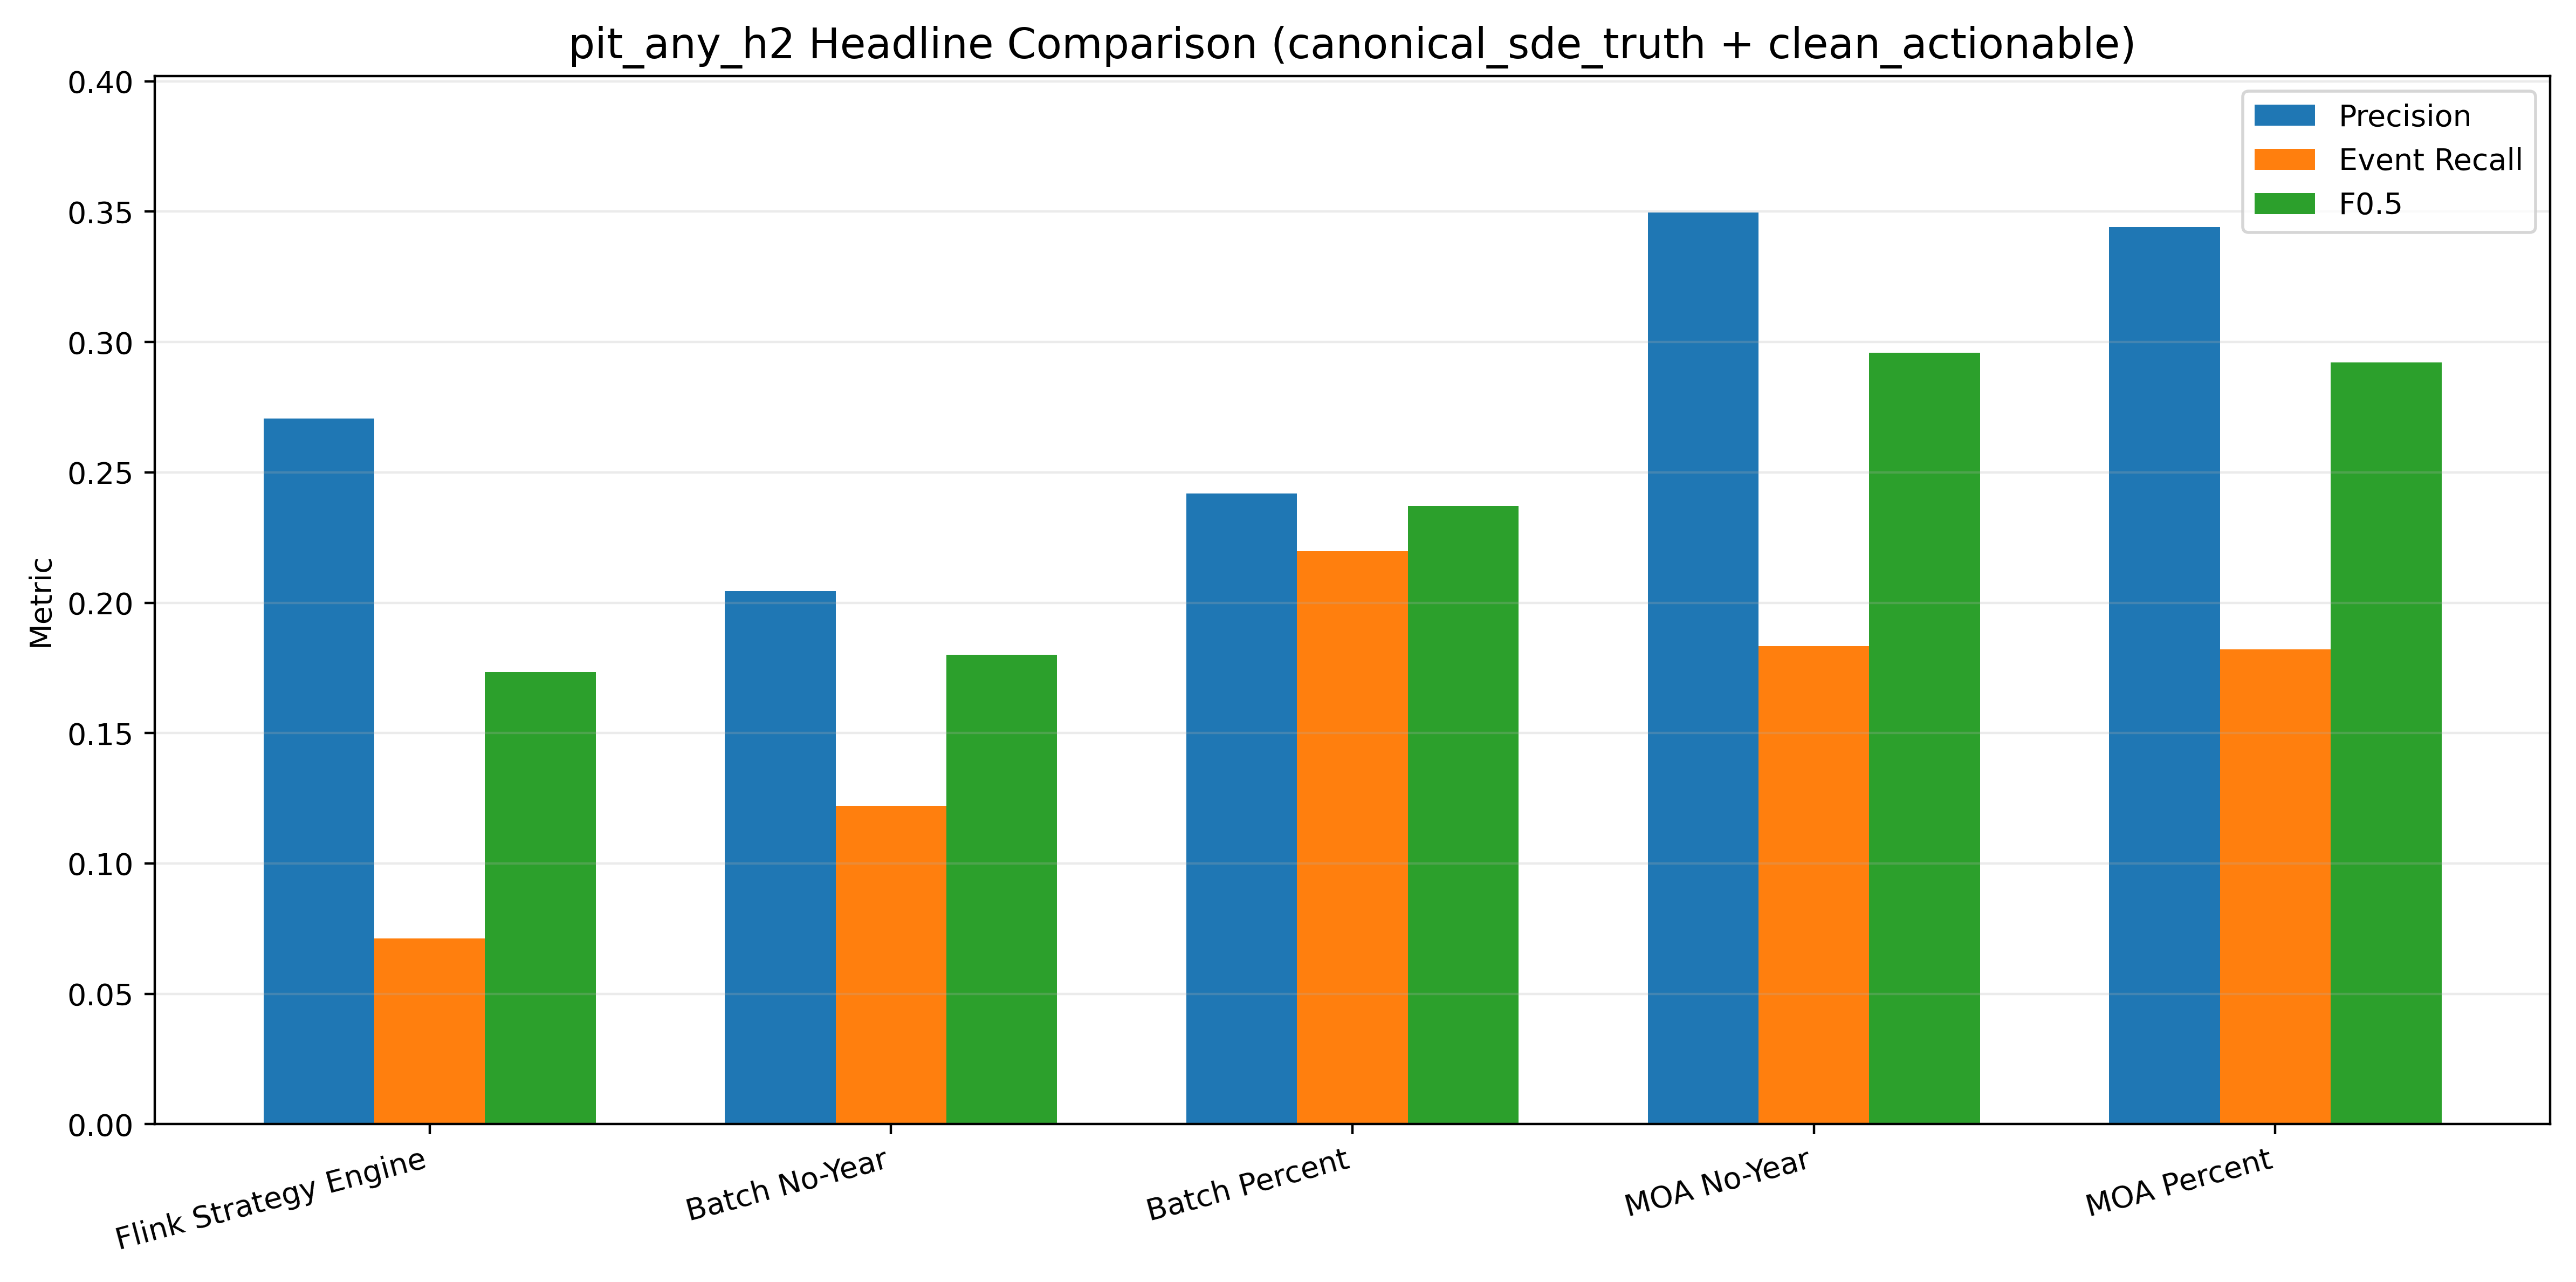
\includegraphics[width=0.99\textwidth]{Images/ch5/pit_any_headline_comparison.png}
    \caption{\texttt{pit\_any\_h2} headline comparison under the \texttt{canonical\_sde\_truth} universe and \texttt{clean\_actionable} lens. The figure
        reports precision, event recall, and $F_{0.5}$ for the selected operating points of the compared systems.}
    \label{fig:pit_any_headline_comparison}
\end{figure}

The visual comparison confirms the same interpretation as Table~\ref{tab:pit_any_interpretation}: learned models improve the timing task over the
deterministic rule baseline, with Batch Percent giving the largest event recall and MOA giving the strongest precision-oriented balance.


\section{Accounting Semantics and \texttt{pit\_success\_h2} Strict Contract}

Before presenting the \texttt{pit\_success\_h2} results, the accounting semantics must be clarified. The success contract is stricter than the pit timing contract because a
positive call is correct only if an eligible future pit happens and that pit is later classified as successful.

This creates a distinction between decision-level quantities and event-level quantities. A system emits positive calls at driver-lap level, while the truth is defined by
pit events and post-pit outcome labels. For this reason, the metrics used in this section do not all have the same denominator. The evaluation separates three quantities:
strict precision, successful event coverage, and matched-pit success rate.

\subsection{Decision-vs-Event Ledger Clarification}

The first quantity is strict precision. This is the main operational precision used for the \texttt{pit\_success\_h2} comparison. A positive call is counted as a true
positive only if it matches an eligible future pit whose outcome is successful. A positive call with no matched pit is counted as a false positive, because the system
still emitted a successful-pit recommendation that did not correspond to an eligible future pit. A positive call matched to a failed or disadvantage pit is also counted
as a false positive. In compact form:

\[
    strictPrecision =
    \frac{TP}{TP + FP_{no\_match} + FP_{failure}}.
\]

The second quantity is successful event coverage, which is an event-level measure. It counts how many eligible successful pit events were covered by at least one positive call.
Its denominator is the number of eligible successful pit events in the truth universe:

\[
    successfulEventCoverage =
    \frac{coveredSuccessfulEvents}{eligibleSuccessfulEvents}.
\]

This quantity is useful because a system can have reasonable precision while still missing most successful pit opportunities.

The third quantity is matched-pit success rate. This is a diagnostic measure only. It considers only the positive calls that matched a known pit event, and then checks how
many of those matched pits were successful:

\[
    matchedPitSuccessRate =
    \frac{matchedSuccess}{matchedSuccess + matchedFailure}.
\]

This value is not the same as operational precision because it ignores positive calls that did not match any eligible pit. It therefore describes the quality of calls after
a pit match has already occurred, but it does not describe the full operational behaviour of the system. For this reason, matched-pit success rate is not used as the main
precision metric in the headline comparison.

The following sections use strict precision and successful event coverage for the main \texttt{pit\_success\_h2} comparison. Matched-pit success rate is kept separate as
a diagnostic quantity.

\subsection{Strict \texttt{pit\_success\_h2} Table and Sensitivity}

Table~\ref{tab:pit_success_selected} reports the selected strict \texttt{pit\_success\_h2} operating points for all compared systems. For the Flink Strategy Engine,
the positive call is the deterministic \texttt{PIT\_NOW} label. For Batch XGBoost and MOA, the positive call is obtained by applying the selected threshold to the model score.

The selected results confirm that \texttt{pit\_success\_h2} is substantially harder than \texttt{pit\_any\_h2}, the Flink Strategy Engine covers more successful events
than the selected learning policies, but it does so by emitting many more positive calls. Once no-match calls and failed matched pits are counted as false positives,
its strict precision is low. The selected learning policies are more conservative: they emit fewer calls, obtain higher strict precision, but cover only a small fraction
of successful pit events.

Among the selected learning policies, MOA Percent obtains the highest strict precision and the best $F_{0.5}$ score. MOA No-Year follows with lower coverage and lower
precision, while the two Batch configurations remain more conservative in terms of emitted calls and successful event coverage.

\begin{table}[htbp]
    \centering
    \caption{Selected strict \texttt{pit\_success\_h2} operating points.}
    \label{tab:pit_success_selected}
    \begin{tabular}{lccccc}
        \toprule
        System                & \shortstack{Threshold                                \\Rule} & Predicted + & \shortstack{Strict\\precision} & \shortstack{Success\\coverage} & $F_{0.5}$ \\
        \midrule
        Flink Strategy Engine & \texttt{PIT\_NOW}     & 1235 & 0.080 & 0.083 & 0.081 \\
        Batch No-Year         & 0.37                  & 46   & 0.239 & 0.010 & 0.044 \\
        Batch Percent         & 0.51                  & 51   & 0.196 & 0.009 & 0.040 \\
        MOA No-Year           & 0.58                  & 52   & 0.288 & 0.014 & 0.059 \\
        MOA Percent           & 0.58                  & 86   & 0.365 & 0.029 & 0.111 \\
        \bottomrule
    \end{tabular}
\end{table}

The selected points are intentionally strict, they show the behaviour of each system under the frozen operating policy. However, the threshold frontier also makes it
possible to inspect how the learned systems behave when the threshold is relaxed. Table~\ref{tab:pit_success_relaxed} reports this sensitivity check for the Percent profiles.

The relaxed rows are diagnostic only since they are not the main headline policy. Their purpose is to show the trade-off between call volume, strict precision, and successful
event coverage. Lowering the threshold increases the number of emitted calls and covers more successful pit events, but it also accepts more false positives. Batch
Percent increases from 51 to 844 positive calls and from $0.009$ to $0.083$ coverage, while precision drops from $0.196$ to $0.105$. MOA Percent increases from 86 to
900 positive calls and from $0.029$ to $0.169$ coverage, while precision drops from $0.365$ to $0.205$.

\begin{table}[htbp]
    \centering
    \caption{Relaxed diagnostic sensitivity points for \texttt{pit\_success\_h2} Percent profiles.}
    \label{tab:pit_success_relaxed}
    \begin{tabular}{lccccc}
        \toprule
        System                & Threshold & Predicted + & \shortstack{Strict                 \\precision} & \shortstack{Success\\coverage} & $F_{0.5}$ \\
        \midrule
        Batch Percent relaxed & 0.22      & 844         & 0.105              & 0.083 & 0.100 \\
        MOA Percent relaxed   & 0.51      & 900         & 0.205              & 0.169 & 0.196 \\
        \bottomrule
    \end{tabular}
\end{table}

Figure~\ref{fig:pit_success_apples_to_apples_main} visualizes the selected strict comparison. The figure highlights the main result of this subsection: \texttt{pit\_success\_h2}
is both rarer and stricter than pit timing, because positive calls are penalized when they do not match an eligible future pit or when the matched pit is not successful.

\begin{figure}[htbp]
    \centering
    
\includegraphics[width=0.95\textwidth]{Images/ch5/pit_success_apples_to_apples_main.png}
    \caption{Strict \texttt{pit\_success\_h2} comparison under the \texttt{canonical\_sde\_truth} universe and \texttt{clean\_actionable} lens. The figure reports strict precision,
        successful event coverage, and $F_{0.5}$ for the selected operating points.}
    \label{fig:pit_success_apples_to_apples_main}
\end{figure}





\section{Flink Strategy Engine: Diagnostic Quality vs Operational Precision}

The Flink Strategy Engine also requires a separate diagnostic view. Its \texttt{PIT\_NOW} calls often match pit stops that are later classified as successful,
but this does not mean that the engine has high operational precision under the strict \texttt{pit\_success\_h2} contract.

The reason is the denominator, matched-pit success rate only considers calls that matched a known pit event. It ignores calls that did not match any eligible future pit.
Strict precision, instead, includes those no-match calls as false positives. Therefore, matched-pit success rate can be high while strict operational precision remains low.

For \texttt{PIT\_NOW}, the matched-pit success rate is $0.583$, while strict precision is $0.080$. When \texttt{GOOD\_PIT} is added to the positive-call definition, the
matched-pit success rate increases to $0.628$, but strict precision decreases to $0.060$. This means that, conditional on matching a pit, many Flink calls correspond to
successful outcomes. However, the engine also emits many calls that do not match an eligible future pit, and those calls reduce operational precision.

\begin{table}[htbp]
    \centering
    \caption{Flink Strategy Engine diagnostic quality versus strict operational precision.}
    \label{tab:sde_diagnostic_vs_operational}
    \begin{tabular}{lcc}
        \toprule
        Positive-call definition               & Matched-pit success rate & Strict precision \\
        \midrule
        \texttt{PIT\_NOW}                      & 0.583                    & 0.080            \\
        \texttt{PIT\_NOW} + \texttt{GOOD\_PIT} & 0.628                    & 0.060            \\
        \bottomrule
    \end{tabular}
\end{table}

Figure~\ref{fig:sde_diagnostic_operational_vs_matched} visualizes the same distinction. The matched-pit success rate is useful for understanding the quality of calls after
a pit match has occurred.

\begin{figure}[htbp]
    \centering
    
\includegraphics[width=0.85\textwidth]{Images/ch5/pit_success_sde_diagnostic_operational_vs_matched.png}
    \caption{Flink Strategy Engine diagnostic matched-pit success rate compared with strict operational precision. Matched-pit success rate is diagnostic only and is not
        the headline precision metric.}
    \label{fig:sde_diagnostic_operational_vs_matched}
\end{figure}


\section{Cross-Task Headline Synthesis}

The two headline tasks show different behaviours, the \texttt{pit\_any\_h2} contract is the cleaner timing task. It only asks whether a pit stop happens soon,
so the systems are evaluated on their ability to recognize an approaching pit window. Under this contract, the learning-based systems improve over the deterministic
Flink Strategy Engine. Batch Percent gives the largest event recall, while MOA provides the strongest precision-oriented balance.

The \texttt{pit\_success\_h2} contract is stricter, a correct positive call must match a future eligible pit and that pit must be classified as successful.
This makes the task sparser and more sensitive to the threshold policy. Under the selected strict operating points, MOA Percent gives the cleanest successful-pit
calls, with the highest strict precision and the best $F_{0.5}$ among the selected learning policies. However, its successful event coverage remains low, which
shows that the task is still difficult even for the best selected learner.

The Flink Strategy Engine plays a different role in the comparison because it remains the interpretable deterministic baseline and emits more calls than the selected
learned policies in the success task. This gives it some successful event coverage, but strict precision is low once no-match calls and failed matched pits are
counted as false positives. At the same time, its matched-pit success rate is useful diagnostically: when a Flink call does match a known pit, many of those
matched pits are successful.

Overall, the results suggest that pit timing is more learnable from the available race context than successful pit-call prediction. The learning branches are
better at ranking and thresholding pit timing situations, while the success contract exposes the harder part of the problem: distinguishing not only when a pit
will happen, but whether that future pit will also be strategically favourable under the post-pit evaluation logic.

\section{PR Curves and Average Precision (Ranking Diagnostics)}

The headline tables report selected operating points, they show what happens after each score-based system has been converted into positive calls through a threshold.
Precision-recall curves provide a complementary view: they inspect how the score behaves across many possible thresholds, before committing to one operating point.

This section therefore treats PR curves and Average Precision as ranking diagnostics. They are useful for understanding whether a model assigns higher scores to positive
rows than to negative rows, and whether a different threshold could expose a better precision-recall trade-off.

\subsection{Diagnostic framing}

Precision-recall curves are computed at row level for score based systems, Batch XGBoost produces probability scores, while MOA produces vote-based scores through the
custom logger described in Chapter~\ref{ch:problem_solving}. By sweeping a threshold over these scores, each system produces a curve showing how precision and recall
change as the positive-call policy becomes more or less aggressive.

Average Precision summarizes this row-level ranking behaviour into a single value. A higher AP means that positive rows tend to receive higher scores than negative rows.
However, AP is not the same as strict operational precision. In particular, for \texttt{pit\_success\_h2}, the headline comparison must still count no-match calls and
failed matched pits as false positives.

The Flink Strategy Engine is different. It does not produce a continuous learned score used for threshold sweeping in the same way as Batch and MOA. It emits deterministic
labels such as \texttt{MONITOR}, \texttt{GOOD\_PIT}, and \texttt{PIT\_NOW}. Therefore, in the PR figures the Flink Strategy Engine is best interpreted as a fixed operating
point rather than as a learned score curve.

The purpose of this section is to inspect whether the learned systems rank the rows in a useful way. The final comparison remains based on the selected thresholds and on
the strict accounting rules defined earlier.


\subsection{PR Figures and AP Table}

Figures~\ref{fig:pr_curve_pit_any_final} and~\ref{fig:pr_curve_pit_success_final} show the precision--recall curves for the two targets,
these plots compare the score-based systems across thresholds, so they are useful for inspecting ranking behaviour before selecting an operating point. The 
Flink Strategy Engine is shown as a fixed operating point, since it emits deterministic labels rather than a continuous learned score curve.

\begin{figure}[htbp]
    \centering
    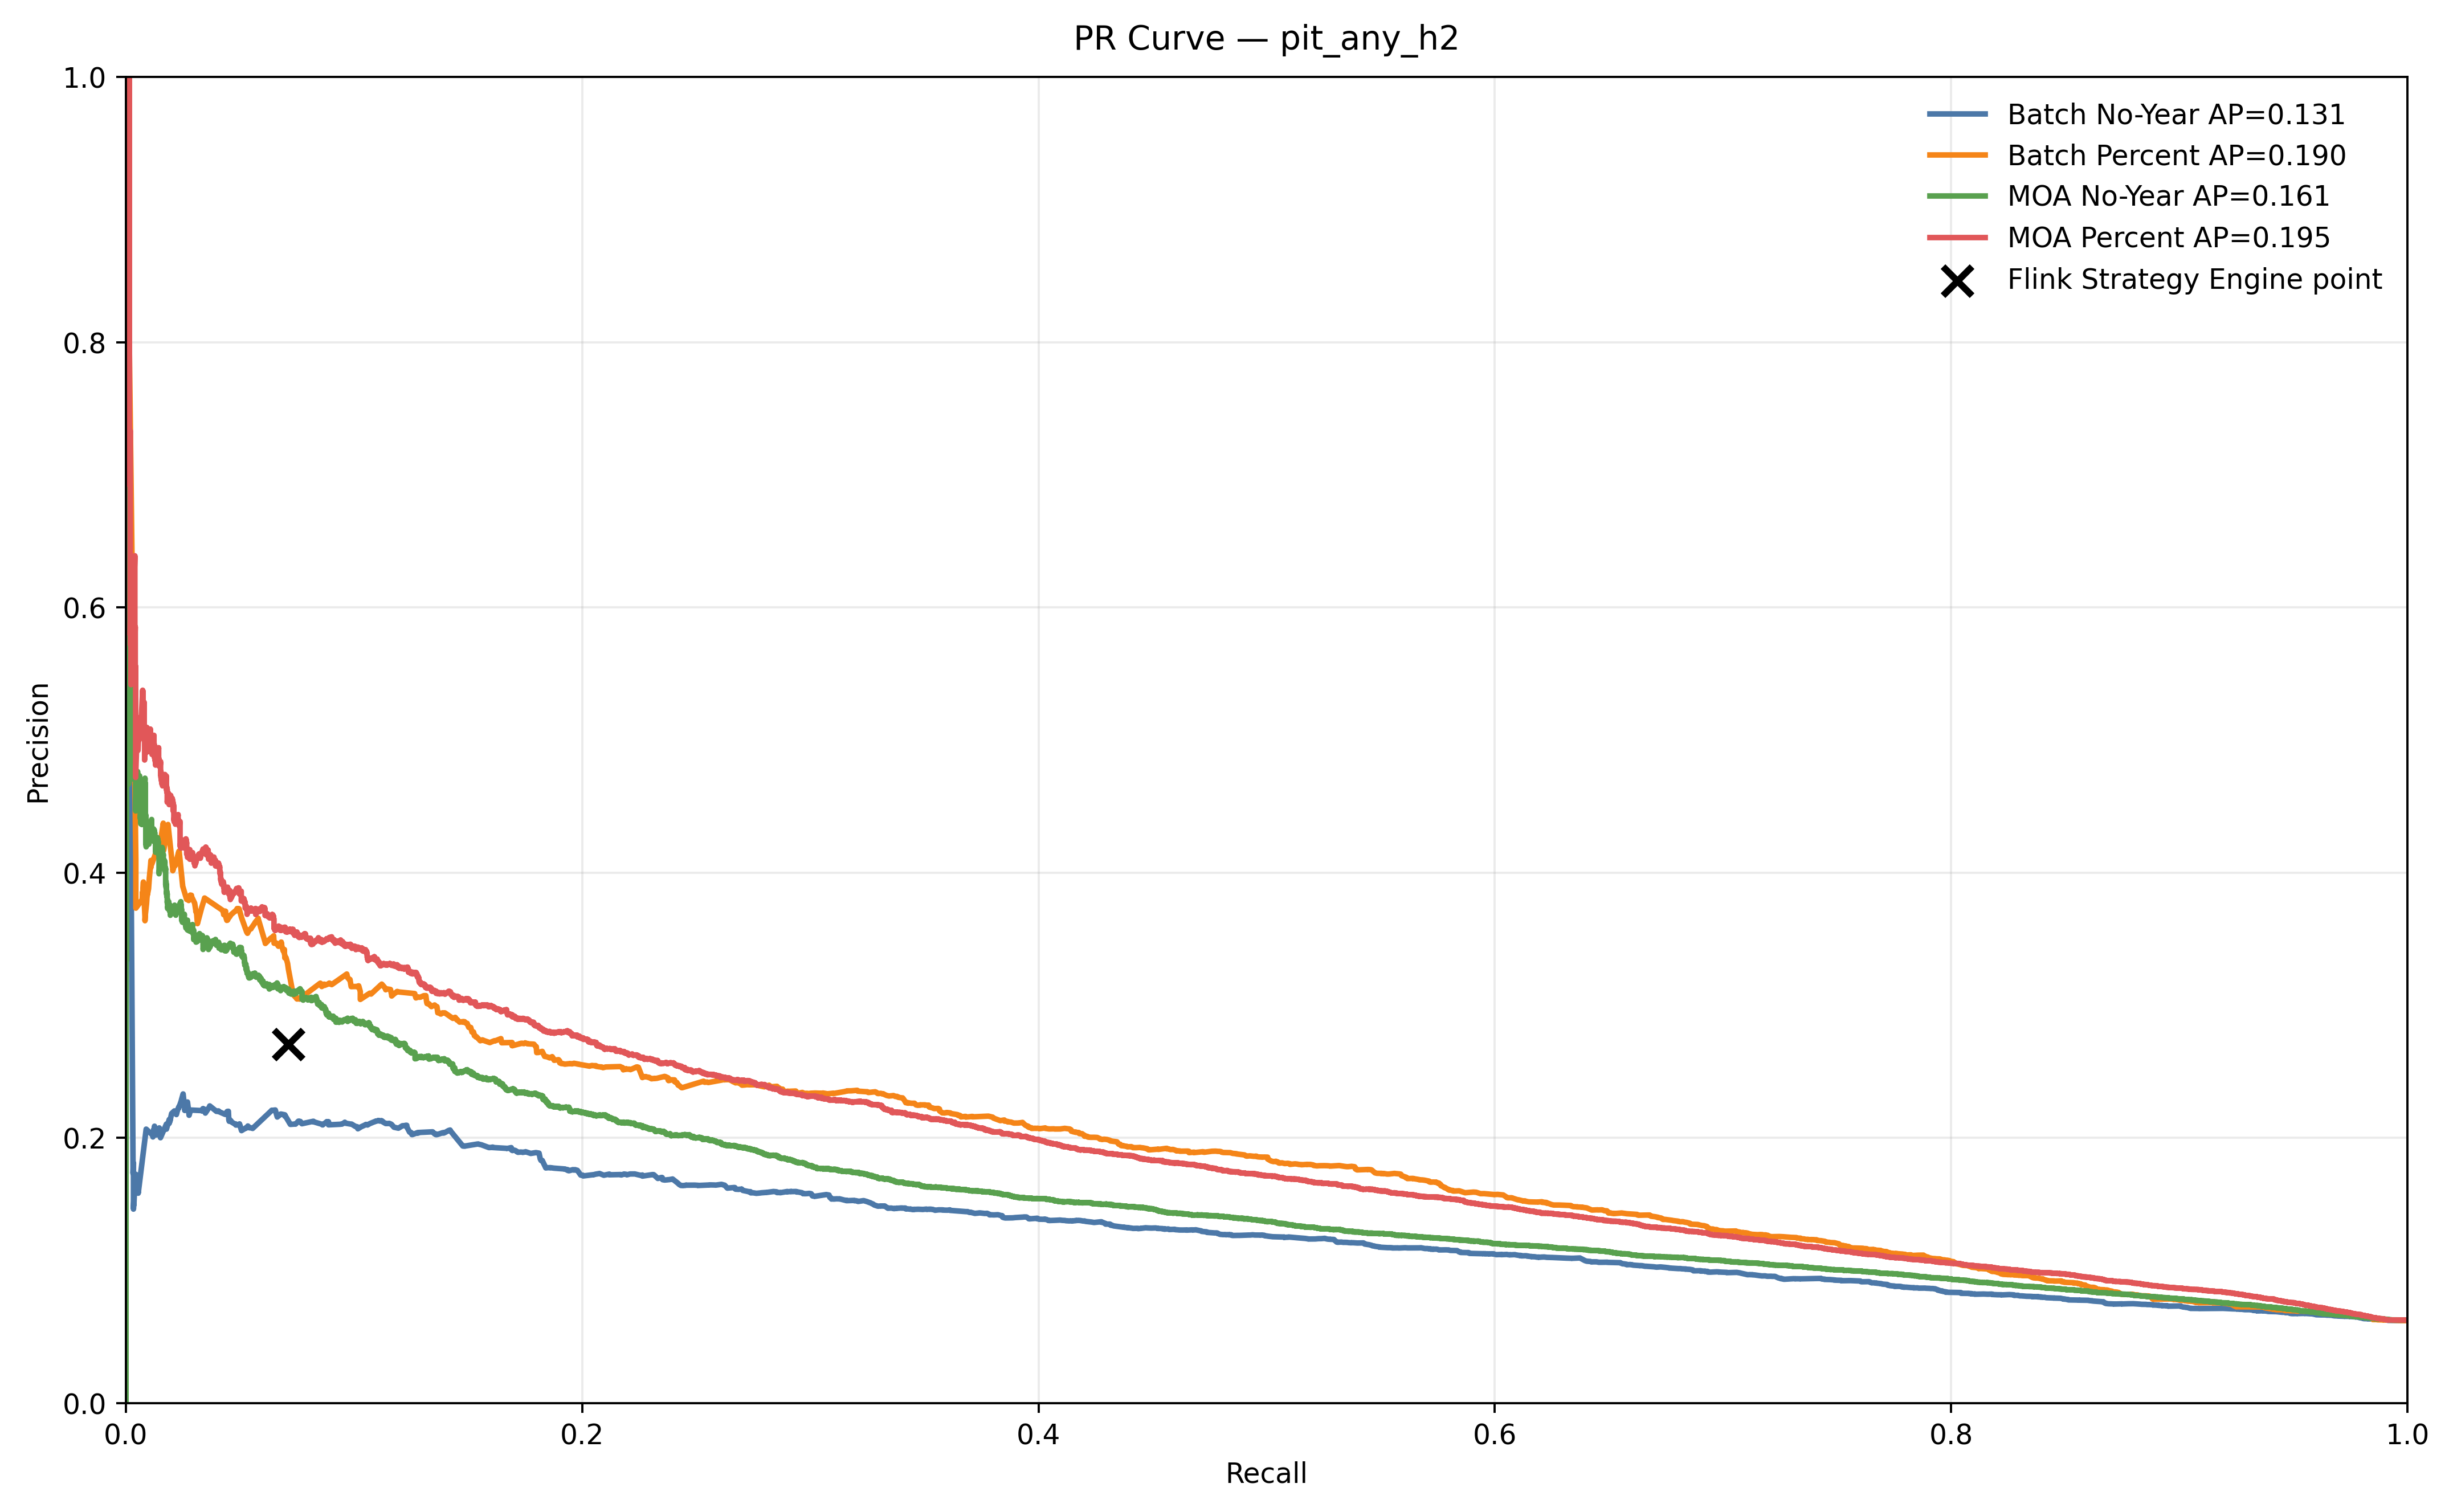
\includegraphics[width=0.85\textwidth]{Images/ch5/pr_curve_pit_any_final.png}
    \caption{Precision--recall curve for \texttt{pit\_any\_h2}.}
    \label{fig:pr_curve_pit_any_final}
\end{figure}

\begin{figure}[htbp]
    \centering
    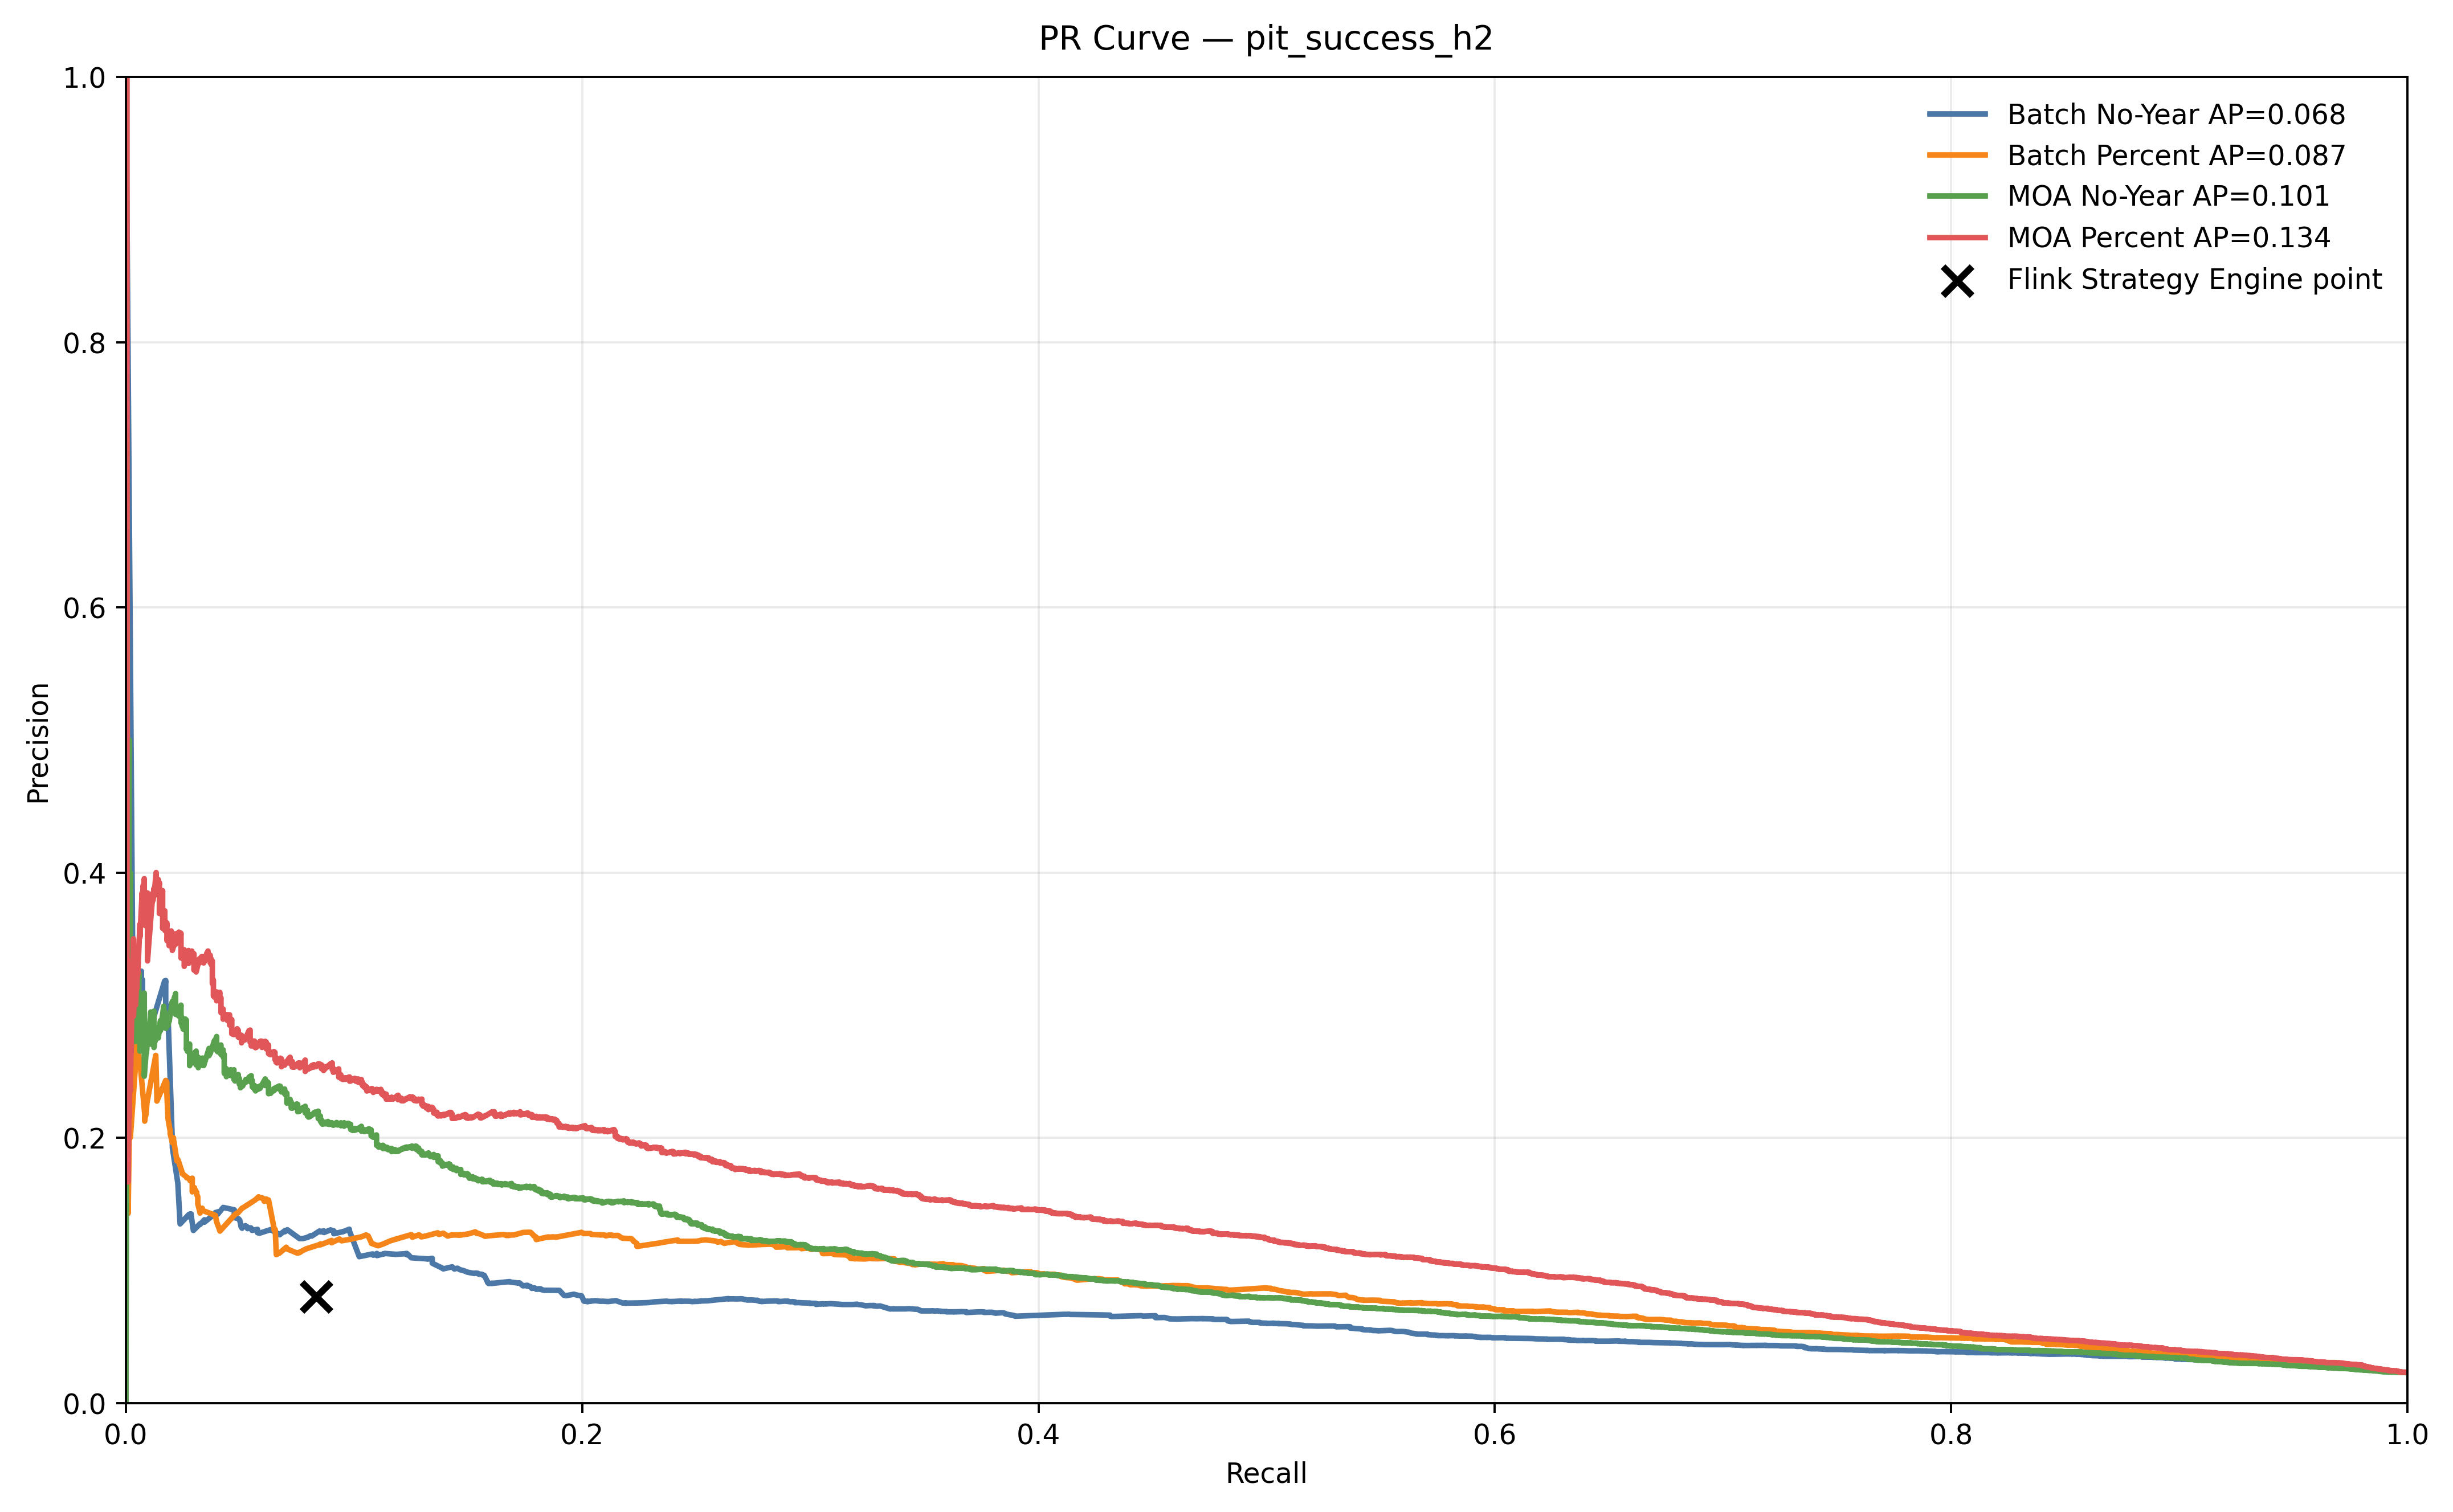
\includegraphics[width=0.85\textwidth]{Images/ch5/pr_curve_pit_success_final.png}
    \caption{Precision--recall curve for \texttt{pit\_success\_h2}.}
    \label{fig:pr_curve_pit_success_final}
\end{figure}

Table~\ref{tab:ap_summary_final} reports Average Precision for the score-based systems. For both targets, MOA Percent obtains the highest AP. 
On \texttt{pit\_any\_h2}, Batch Percent is close to MOA Percent, which is consistent with the strong timing behaviour already observed in the 
selected operating points. On \texttt{pit\_success\_h2}, the AP values are lower overall, confirming that the success task is harder to rank 
as well as harder to classify under a fixed threshold.

\begin{table}[htbp]
    \centering
    \caption{Average Precision for score-based systems. AP is a row-level ranking diagnostic, not operational precision.}
    \label{tab:ap_summary_final}
    \begin{tabular}{lcccc}
        \toprule
        Target                  & Batch No-Year & Batch Percent & MOA No-Year & MOA Percent \\
        \midrule
        \texttt{pit\_any\_h2}     & 0.131         & 0.190         & 0.161       & 0.195 \\
        \texttt{pit\_success\_h2} & 0.068         & 0.087         & 0.101       & 0.134 \\
        \bottomrule
    \end{tabular}
\end{table}

The AP table should be read together with the headline metrics. A model can have a useful ranking curve while still requiring a conservative threshold 
to obtain acceptable operational precision. This is especially visible for \texttt{pit\_success\_h2}, where the best AP belongs to 
MOA Percent, but the selected operating point still has low successful event coverage.

\section{Support-Aware Race-Level Diagnostics}

\subsection{\texttt{pit\_any\_h2}: Kappa and G-Mean per race}

% Slide 53 (Kappa) + Slide 54 (G-Mean).
%
% Goal:
% Show race-level variability under minimum positive support filtering.
%
% Verified support filter and kept races:
% \begin{itemize}
%     \item positives\_min\_filter = 3.
%     \item pit\_any: Flink 92, Batch No-Year 91, Batch Percent 91, MOA No-Year 92, MOA Percent 92.
% \end{itemize}
%
% Artifact anchors:
% \begin{itemize}
%     \item \path{data_lake/reports/phase2b_presentation_figures/final_refresh/race_level_kappa_pit_any.png}
%     \item \path{data_lake/reports/phase2b_presentation_figures/final_refresh/race_level_gmean_pit_any.png}
%     \item \path{data_lake/reports/phase2b_presentation_figures/final_refresh/race_level_support_summary.csv}
% \end{itemize}

\subsection{\texttt{pit\_success\_h2}: Kappa and G-Mean per race}

% Slide 55 (Kappa) + Slide 56 (G-Mean).
%
% Goal:
% Show that strict pit-success race-level diagnostics are much sparser and often near zero.
%
% Verified support filter and kept races:
% \begin{itemize}
%     \item positives\_min\_filter = 3.
%     \item pit\_success: Flink 87, Batch No-Year 86, Batch Percent 86, MOA No-Year 87, MOA Percent 87.
% \end{itemize}
%
% Artifact anchors:
% \begin{itemize}
%     \item \path{data_lake/reports/phase2b_presentation_figures/final_refresh/race_level_kappa_pit_success.png}
%     \item \path{data_lake/reports/phase2b_presentation_figures/final_refresh/race_level_gmean_pit_success.png}
%     \item \path{data_lake/reports/phase2b_presentation_figures/final_refresh/race_level_metric_summary.csv}
% \end{itemize}
%
% Writing caution:
% \begin{itemize}
%     \item treat Kappa/G-Mean as diagnostics (support-sensitive), not headline metrics.
% \end{itemize}


\section{Explainability as Methodology Debugging}
\label{sec:explainability}

\subsection{Explainability role across systems}

% Slide 57.
%
% Goal:
% Explain why explainability is presented as debugging/interpretation support.
%
% Slide-grounded content to keep:
% \begin{itemize}
%     \item Batch XGBoost: direct SHAP / TreeSHAP on trained model.
%     \item MOA Online Learner: surrogate SHAP proxy.
%     \item Flink Strategy Engine: rule logic is interpretable by construction.
% \end{itemize}
%
% Important consistency line:
% \begin{itemize}
%     \item this section supports methodological choices (e.g., No-Year correction), not claims of causal feature effects.
% \end{itemize}

\subsection{\texttt{\_source\_year} shortcut-risk and No-Year correction}

% Slide 58 + Slide 59.
%
% Goal:
% Link explainability findings to protocol corrections already described in Chapter 4.
%
% Slide-grounded claims to keep:
% \begin{itemize}
%     \item \texttt{\_source\_year} appeared as shortcut-risk in Batch explainability.
%     \item this motivated No-Year as the clean neutral baseline.
%     \item Percent profile is engineered, not a fully neutral comparison.
% \end{itemize}
%
% Provenance note (important):
% \begin{itemize}
%     \item Current \texttt{final\_refresh/} package contains the corrected evaluation tables/figures but does not include a dedicated SHAP CSV set.
%     \item If the SHAP comparison figure from Slide 59 is inserted in thesis, add explicit provenance to the exact image-generation artifact used (currently available in local archive history).
% \end{itemize}
%
% TODO: add reproducible explainability artifact path (or regenerate into a tracked thesis-facing location before final submission).


\section{Threats to Validity}

% Map to the closing cautionary points embedded across Slides 50--59.
%
% Threats to include:
% \begin{itemize}
%     \item support sparsity and race-level volatility (especially strict pit\_success).
%     \item threshold-policy dependence for operational behavior.
%     \item comparator-contract dependence (window semantics and unknown handling).
%     \item surrogate explainability limits for online learners.
% \end{itemize}
%
% Suggested anchors:
% \begin{itemize}
%     \item \path{data_lake/reports/phase2b_presentation_figures/final_refresh/race_level_support_summary.csv}
%     \item \path{data_lake/reports/phase2b_presentation_figures/final_refresh/pit_success_threshold_sensitivity_slide.csv}
%     \item \path{data_lake/reports/phase2b_presentation_figures/final_refresh/final_slide_assets_manifest.csv}
% \end{itemize}


% Writing rule for Chapter 5:
% Every numeric claim must be traceable to a file under
% \path{data_lake/reports/phase2b_presentation_figures/final_refresh/}
% or to an explicitly cited upstream source listed in
% \path{data_lake/reports/phase2b_presentation_figures/final_refresh/final_refresh_input_provenance.csv}.
